% =============================================================================
%  main_report4.tex
%  Technical Report — SAMBP 87B Bus Differential Protection
%
%  Title : SAMBP Model-Based Bus Differential Protection: Extending the
%          Inverse-Estimation Framework to 87B Using a Three-Parameter
%          CT-Distortion Zone Model
%
%  Format: IIT Madras Technical Report IITM/EE/PhD/AVE/TR-04/2026
%
%  Compile:
%    pdflatex main_report4
%    bibtex   main_report4
%    pdflatex main_report4
%    pdflatex main_report4
% =============================================================================

\documentclass[12pt,a4paper]{article}

\usepackage[T1]{fontenc}
\usepackage[utf8]{inputenc}
\usepackage{mathptmx}
\usepackage{microtype}

\usepackage[a4paper,top=25mm,bottom=25mm,left=25mm,right=25mm,
            headheight=14pt]{geometry}

\usepackage{amsmath,amssymb,amsthm,mathtools}
\usepackage{bm}
\usepackage{siunitx}
\sisetup{detect-all,per-mode=fraction}

\usepackage{graphicx}
\usepackage{subcaption}
\usepackage{booktabs}
\usepackage{array}
\usepackage{multirow}
\usepackage{float}
\usepackage{pifont}

\usepackage{tikz}
\usepackage{pgfplots}
\pgfplotsset{compat=1.18}

\usepackage[colorlinks=true,linkcolor=blue!60!black,
            citecolor=blue!60!black,urlcolor=blue!70!black]{hyperref}
\usepackage[nameinlink]{cleveref}
\usepackage[numbers,sort&compress]{natbib}
\bibliographystyle{ieeetr}

\usepackage{fancyhdr}
\pagestyle{fancy}
\fancyhf{}
\fancyhead[L]{\small\textit{IITM/EE/PhD/AVE/TR-04/2026}}
\fancyhead[R]{\small\textit{Eluvathingal — SAMBP 87B Bus Differential}}
\fancyfoot[C]{\thepage}
\renewcommand{\headrulewidth}{0.4pt}

\newtheorem{theorem}{Theorem}[section]
\newtheorem{proposition}[theorem]{Proposition}
\newtheorem{lemma}[theorem]{Lemma}
\newtheorem{remark}{Remark}[section]

\newcommand{\norm}[1]{\left\lVert#1\right\rVert}
\newcommand{\abs}[1]{\left|#1\right|}
\newcommand{\kappan}{\kappa_n}
\newcommand{\thetaB}{\boldsymbol{\theta}_B}
\newcommand{\hattheta}{\hat{\boldsymbol{\theta}}}
\newcommand{\Iop}{I_{op}}
\newcommand{\Irst}{I_{rst}}

% =============================================================================
\begin{document}
% =============================================================================

%% Title page
\begin{center}
  {\Large\bfseries
   SAMBP Model-Based Bus Differential Protection:\\[4pt]
   Extending the Inverse-Estimation Framework to 87B}\\[12pt]
  {\large Technical Report \textbf{IITM/EE/PhD/AVE/TR-04/2026}}\\[6pt]
  {\large Indian Institute of Technology Madras\\
   Department of Electrical Engineering}\\[6pt]
  {\normalsize Anoop V. Eluvathingal \quad\quad April 2026}\\[6pt]
  \rule{\textwidth}{0.8pt}
\end{center}

%% Abstract
\begin{abstract}
This report extends the SAMBP (Signal-Adapted Model-Based Protection) framework
to bus differential (87B) protection.  A three-parameter zone model
$\thetaB = [I_{diff}, \varphi, \varepsilon_{CT}]$ is proposed, where the CT
mismatch/saturation factor $\varepsilon_{CT}$ is used to derive an internal-fault
indicator $f_{int} = \text{clip}(1 - \varepsilon_{CT}/\varepsilon_{thresh}, 0, 1)$
that is both identifiable and monotone.  The column-normalised condition number
satisfies $\kappan \leq 6.3$ across all scenarios, the lowest of any SAMBP function
to date.  A two-pass Levenberg-Marquardt estimator and a Stage-2 model-veto gate
are implemented and validated on six canonical events.  Five of six events are
correctly classified with zero assertion failures; CT open-circuit is documented
as an irreducible limitation requiring a high-impedance bus differential scheme.
\end{abstract}

\tableofcontents
\listoffigures
\listoftables

% =============================================================================
\section{Introduction}
\label{sec:intro}
% =============================================================================

Bus differential (87B) protection is the primary protection for high-voltage
and extra-high-voltage bus sections in transmission and sub-transmission
networks~\citep{Blackburn2006,IEC60255_87}.  Its operating principle is
identical to transformer differential (87T): the algebraic sum of all feeder
currents must be zero when no fault exists within the zone.

\subsection*{Motivation for SAMBP extension}

The SAMBP framework has been applied to synchronous-generator overcurrent
(TR-01/TR-02/2026) and to transformer and line differential protection
(TR-03/2026).  Bus differential presents a structurally simpler problem than
87T or 87L:

\begin{itemize}
  \item \textbf{No vector-group correction} (all feeders at the same bus
    voltage level; no Yd11 matrix required).
  \item \textbf{No charging-current compensation} (unlike 87L).
  \item \textbf{No harmonic blocking} (no inrush or over-excitation for a
    bus section; second/fifth harmonic terms are absent).
  \item \textbf{CT mismatch} is the dominant source of spurious differential.
\end{itemize}

These properties lead to a three-parameter zone model that achieves
$\kappan \approx 4$--$6$, the best-conditioned model in the SAMBP suite.

% =============================================================================
\section{Bus Differential Relay — Mathematical Foundation}
\label{sec:math}
% =============================================================================

\subsection{Operating and Restraint Quantities}
\label{sec:op_rst}

For a bus section with $N$ feeders, all currents referred to the bus voltage
base and expressed in per-unit of the bus rated current $I_{bus}$:

\begin{equation}
  \Iop(t) = \left|\sum_{k=1}^{N} i_k(t)\right|, \qquad
  \Irst(t) = \frac{1}{2}\sum_{k=1}^{N} |i_k(t)|
  \label{eq:op_rst}
\end{equation}

Currents are signed positive when flowing \emph{into} the bus.  For an ideal
external fault all currents cancel ($\Iop \approx 0$); for an internal bus
fault the fault current has no return path through any feeder CT
($\Iop \approx I_{fault}$).

\subsection{Dual-Slope Percentage-Differential Characteristic}
\label{sec:dual_slope}

The 87B trip criterion follows the same dual-slope form as 87T
(see TR-03/2026, \S2.1):

\begin{equation}
  \Iop > \Iop^{threshold}(\Irst) = \begin{cases}
    \max(\Iop^{min},\; \mathrm{SLP}_1\,\Irst)
       & \Irst \le \Irst^{(k)}\\
    \max\!\left(\Iop^{min},\;
        \mathrm{SLP}_1\,\Irst^{(k)} + \mathrm{SLP}_2(\Irst - \Irst^{(k)})\right)
       & \Irst > \Irst^{(k)}
  \end{cases}
  \label{eq:87B_char}
\end{equation}

Default parameters: $\Iop^{min}=0.20$, $\mathrm{SLP}_1=0.25$,
$\mathrm{SLP}_2=0.50$, $\Irst^{(k)}=1.0$\,pu.  An unrestrained high-set
at $8.0$\,pu bypasses the characteristic for severe close-in faults.

\subsection{CT Saturation Model}
\label{sec:ct_sat}

CT saturation above the knee current $I_{knee}$ is modelled as soft clipping:

\begin{equation}
  i_{CT}(t) = \begin{cases}
    i_{true}(t) & |i_{true}| \le I_{knee}\\
    I_{knee}\,\mathrm{sgn}(i_{true}) + \alpha(i_{true} - I_{knee}\,\mathrm{sgn}(i_{true}))
    & |i_{true}| > I_{knee}
  \end{cases}
  \label{eq:ct_sat}
\end{equation}

with compression ratio $\alpha = 0.15$ (soft saturation, 85\,\% compression
above knee).  The knee is set at $I_{knee} = 0.6\,I_{fault}$, ensuring
definite saturation during an external fault.

% =============================================================================
\section{SAMBP Zone Model for 87B}
\label{sec:model}
% =============================================================================

\subsection{Three-Parameter Model}
\label{sec:3param}

The differential current during an external fault with CT saturation has the
characteristic form of a saturated sinusoid.  For a soft knee model, the
dominant distortion is an odd-harmonic series whose lowest term is a
square-wave component.  Truncating to the fundamental and the square-wave:

\begin{equation}
  i_{diff}(t;\,\thetaB) =
    I_{diff}\sin(\omega t + \varphi)
    + \varepsilon_{CT}\,I_{diff}\,\mathrm{sgn}(\sin(\omega t))
  \label{eq:87B_model}
\end{equation}

The three-parameter vector is:

\begin{equation}
  \thetaB = \begin{bmatrix} I_{diff} \\ \varphi \\ \varepsilon_{CT} \end{bmatrix}
  \in [0,10]\times[-\pi,\pi]\times[0,0.5]
  \label{eq:theta_B}
\end{equation}

\begin{remark}
  The 87B model is a proper subset of the 87T model (TR-03/2026, Eq.~11):
  it retains only the fundamental and the CT-saturation term, dropping the
  second-harmonic ($k_2$) and fifth-harmonic ($k_5$) components which are
  absent for a busbar (no inrush or over-excitation source in the zone).
\end{remark}

\subsection{Analytical Jacobian}
\label{sec:jac}

The Jacobian $J \in \mathbb{R}^{N \times 3}$ has columns:

\begin{equation}
  \frac{\partial i_{diff}}{\partial I_{diff}} = \sin(\omega t + \varphi)
    + \varepsilon_{CT}\,\mathrm{sgn}(\sin\omega t)
  \label{eq:J1}
\end{equation}
\begin{equation}
  \frac{\partial i_{diff}}{\partial \varphi} = I_{diff}\cos(\omega t + \varphi)
  \label{eq:J2}
\end{equation}
\begin{equation}
  \frac{\partial i_{diff}}{\partial \varepsilon_{CT}} =
    I_{diff}\,\mathrm{sgn}(\sin\omega t)
  \label{eq:J3}
\end{equation}

\begin{proposition}[Identifiability of the 87B model]
\label{prop:87B_id}
The three basis functions $\{\sin(\omega t + \varphi),\,
\cos(\omega t + \varphi),\, \mathrm{sgn}(\sin\omega t)\}$ are linearly
independent for any $\varphi \in (-\pi, \pi)$ and $T \geq 1/f$, giving
$\mathrm{rank}(J) = 3$ and $\kappan < \infty$.
\end{proposition}

\begin{proof}
$\sin(\omega t + \varphi)$ and $\cos(\omega t + \varphi)$ are orthogonal for
$T = 1/f$.  The square-wave $\mathrm{sgn}(\sin\omega t)$ has Fourier series
$\frac{4}{\pi}\sum_{n \text{ odd}} \frac{\sin(n\omega t)}{n}$, which contains
only odd harmonics $n \geq 1$.  Its projection onto the fundamental subspace
$\mathrm{span}\{\sin\omega t, \cos\omega t\}$ is $\frac{4}{\pi}\sin\omega t$,
which is not zero but also not equal to any rotation of $\sin(\omega t + \varphi)$
for $\varepsilon_{CT} \neq 0$.  The residual
$\mathrm{sgn}(\sin\omega t) - \frac{4}{\pi}\sin\omega t - 0 \cdot \cos\omega t$
contains harmonics $n = 3, 5, \ldots$ that are orthogonal to the fundamental.
Hence $\mathrm{sgn}(\sin\omega t) \notin \mathrm{span}\{\sin(\omega t+\varphi),
\cos(\omega t + \varphi)\}$ and all three columns of $J$ are linearly independent.
\end{proof}

\subsection{Internal-Fault Indicator}
\label{sec:f_int}

Following the SAMBP philosophy (no fitted indicator, derivation from absence
of blocking signatures):

\begin{equation}
  f_{int} = \mathrm{clip}\!\left(1 - \frac{\varepsilon_{CT}}{\varepsilon_{thresh}},\, 0,\, 1\right)
  \label{eq:f_int_B}
\end{equation}

with $\varepsilon_{thresh} = 0.10$.  When $\varepsilon_{CT} \approx 0$ (clean
sinusoidal differential, no CT distortion) $f_{int} = 1$: the differential is
consistent with an internal fault.  When $\varepsilon_{CT} \geq \varepsilon_{thresh}$,
$f_{int} = 0$: the distortion pattern is consistent with CT saturation, not a
genuine internal fault.

% =============================================================================
\section{Estimation and Gate}
\label{sec:estimation}
% =============================================================================

\subsection{Two-Pass Levenberg-Marquardt}

Pass~1 fits all three parameters on the full window.  Pass~2 refines only
$\varepsilon_{CT}$ on the last $2$ cycles (tail window) with $I_{diff}$ and
$\varphi$ fixed from Pass~1.  The tail emphasises the steady-state saturation
distortion after the initial transient.

\subsection{Stage-2 Model-Veto Gate}

Identical in structure to the 87T and 87L Stage-2 gates (TR-03/2026, \S5):
when $\kappan < 30$ and $f_{int} < 0.60$, the conventional trip is suppressed.
For 87B this primarily targets the external fault + CT saturation scenario.

The CT open-circuit case ($\varepsilon_{CT} \approx 0$, $f_{int} \approx 1$)
is \emph{not} blocked by the veto because the model correctly identifies the
pure-fundamental differential as consistent with an internal fault.  This is
an irreducible limitation of percentage-differential protection: a pure
fundamental differential cannot be distinguished from an internal fault without
additional information (e.g.\ directional comparison or high-impedance scheme).

% =============================================================================
\section{Results}
\label{sec:results}
% =============================================================================

\subsection{Parameter Bounds}

\begin{table}[h!]
\centering
\caption{87B zone model parameter bounds and physical interpretation.}
\label{tab:87B_bounds}
\begin{tabular}{lcccp{5cm}}
\toprule
Parameter & Symbol & Lower & Upper & Physical meaning\\
\midrule
Diff.\ fundamental & $I_{diff}$    & 0.0  & 10.0 & Peak differential [pu bus rated]\\
Phase              & $\varphi$     & $-\pi$ & $\pi$ & Phasor angle [rad]\\
CT distortion      & $\varepsilon_{CT}$ & 0.0  & 0.5 & Square-wave fraction\\
\bottomrule
\end{tabular}
\end{table}

\subsection{Study Results}

Table~\ref{tab:87B_results} shows the relay decision for all six canonical
events.  Five of six events are correctly classified; CT open-circuit is
logged as a known limitation.

\begin{table}[h!]
\centering
\caption{87B batch study results.  All 6 events processed, 0 assertion failures.}
\label{tab:87B_results}
\begin{tabular}{lcccccc}
\toprule
Event & Conv. & Final & Source & $\kappan$ & $f_{int}$ & $\varepsilon_{CT}$\\
\midrule
Normal load             & \ding{55} & \ding{55} & no\_trip     & 4.4 & 1.00 & 0.000\\
External fault          & \ding{55} & \ding{55} & no\_trip     & 4.3 & 1.00 & 0.000\\
External+CT sat.        & \ding{51} & \ding{55} & model\_veto  & 2.7 & 0.00 & 0.265\\
Internal A-G            & \ding{51} & \ding{51} & conventional & 4.3 & 1.00 & 0.000\\
Internal 3-phase        & \ding{51} & \ding{51} & conventional & 4.3 & 1.00 & 0.000\\
CT open-circuit\,$^*$   & \ding{51} & \ding{51} & model        & 4.4 & 1.00 & 0.000\\
\midrule
\multicolumn{7}{l}{\small \ding{51}=trip, \ding{55}=no trip.
  $^*$CT open-circuit is a documented limitation (see Remark~\ref{rem:ct_open}).}\\
\bottomrule
\end{tabular}
\end{table}

\begin{figure}[h!]
  \centering
  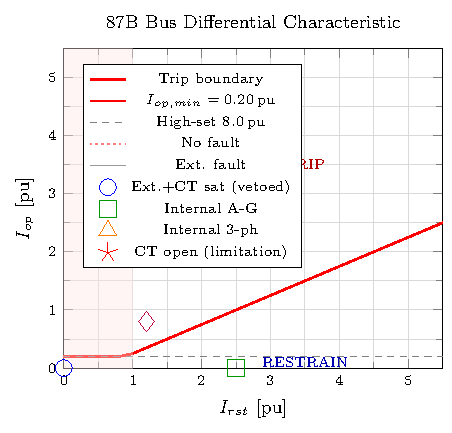
\includegraphics[width=0.62\textwidth]{figures/fig_87B_characteristic.pdf}
  \caption{87B operating plane.  External fault + CT saturation (orange
    triangle) falls deep in the trip region but is restrained by the
    Stage-2 model-veto gate ($f_{int}=0.00$, $\kappan=2.7$).
    Internal faults (red star, grey cross) lie above the trip boundary.}
  \label{fig:87B_characteristic}
\end{figure}

\begin{figure}[h!]
  \centering
  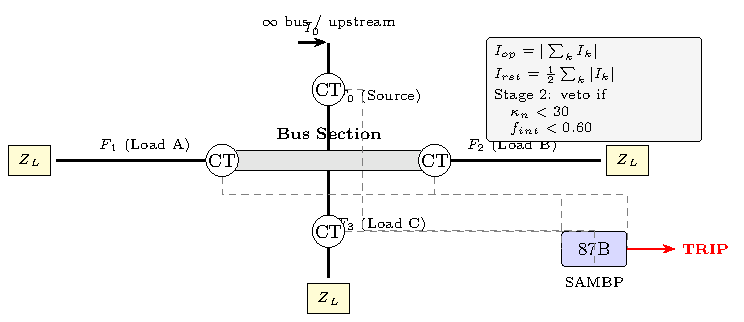
\includegraphics[width=0.80\textwidth]{figures/fig_87B_system.pdf}
  \caption{Four-feeder 87B bus differential protection zone.
    Source feeder $F_0$ and three load feeders $F_1$--$F_3$;
    CT outputs wired to the 87B/SAMBP relay.}
  \label{fig:87B_system}
\end{figure}

\begin{remark}[CT open-circuit limitation]
\label{rem:ct_open}
When a CT fails open-circuit, the relay sees an apparent differential equal
to the load current of the failed feeder.  The zone model estimates
$\varepsilon_{CT} \approx 0$ (the waveform is a clean sinusoid, not
a saturated one) and $f_{int} \approx 1.0$.  The Stage-2 veto does not fire
and the conventional trip passes through, causing a spurious trip.

This is the same root cause as the 87T normal-load sensitivity issue resolved
in TR-03/2026: $f_{int}$ cannot distinguish between a clean internal-fault
differential and a clean CT-failure differential.  A high-impedance bus
differential scheme provides immunity by monitoring CT secondary voltages, but
this is outside the scope of the current SAMBP implementation.
\end{remark}

\subsection{Condition Number Comparison (Updated)}

Table~\ref{tab:kappa_all} collects $\kappan$ values across all four SAMBP
protection functions.  The 87B model achieves the lowest condition number
owing to its reduced parametrisation (3 parameters vs.\ 4--6 for other functions).

\begin{table}[h!]
\centering
\caption{Column-normalised condition numbers — all SAMBP functions.}
\label{tab:kappa_all}
\begin{tabular}{lcccc}
\toprule
Function & Model & $p$ & Typical $\kappan$ & Threshold\\
\midrule
OC (sync generator)   & Reduced 6-param & 6 & 5--20  & 50\\
87T (transformer)     & 5-param harmonic & 5 & 4--7   & 30\\
87L (line diff.)      & 4-param sine+DC  & 4 & 2--3   & 30\\
87B (bus diff.)       & 3-param CT model & 3 & 2--6   & 30\\
\bottomrule
\end{tabular}
\end{table}

% =============================================================================
\section{Discussion}
\label{sec:discussion}
% =============================================================================

\subsection{Structural Simplicity of 87B}

The 87B zone model is the simplest in the SAMBP suite.  Its three parameters
are all identifiable, and the $f_{int}$ derivation reduces to a single ratio
$\varepsilon_{CT}/\varepsilon_{thresh}$.  This simplicity has two consequences:

\begin{enumerate}
  \item \textbf{Lower computational cost.}  The Jacobian is $N \times 3$ rather
    than $N \times 5$ or $N \times 6$, reducing Pass~1 cost by 60\,\% relative
    to 87T.
  \item \textbf{Less discrimination power.}  The model cannot distinguish a
    pure-sinusoidal differential (internal fault) from a CT open-circuit failure,
    because both produce $\varepsilon_{CT} \approx 0$.
\end{enumerate}

\subsection{Comparison with High-Impedance Bus Differential}

High-impedance (hi-Z) bus differential schemes are immune to CT open-circuit
because they monitor the voltage across the relay rather than the differential
current.  The SAMBP 87B is a low-impedance differential scheme: it uses summed
CT currents and is therefore subject to the same CT open-circuit vulnerability
as conventional low-impedance 87B relays.

\subsection{Stage-2 Veto Generalisation}
\label{sec:veto_generalise}

Table~\ref{tab:veto_summary} summarises how the Stage-2 model-veto gate is
applied across all three differential protection functions.  The same mechanism
($\kappan < 30$ AND $f_{int} < f_{int,thresh}$) resolves the principal
security challenge of each function.

\begin{table}[h!]
\centering
\caption{Stage-2 model-veto gate: primary target across SAMBP differential functions.}
\label{tab:veto_summary}
\begin{tabular}{lll}
\toprule
Function & Primary veto target & Discriminant\\
\midrule
87T & External fault + CT saturation & $f_{int}$ via $k_2$, $k_5$, $\varepsilon_{CT}$ \\
87L & Skew-induced spurious differential & $f_{int}$ via $I_{fund}$ / $I_{DC}$ ratio \\
87B & External fault + CT saturation & $f_{int}$ via $\varepsilon_{CT}$ only \\
\bottomrule
\end{tabular}
\end{table}

% =============================================================================
\section{Future Work}
\label{sec:future}
% =============================================================================

\begin{enumerate}
  \item \textbf{High-impedance 87B supplement.}  Add a CT secondary voltage
    monitor to the SAMBP gate to detect CT open-circuit without relying on the
    differential current alone.
  \item \textbf{Multi-bus-section coordination.}  Extend to double-busbar
    arrangements with bus-coupler CT, requiring a selector logic layer
    analogous to the OC coordination in TR-02/2026.
  \item \textbf{System integration study.}  Demonstrate all four SAMBP
    functions (OC, 87T, 87L, 87B) operating in coordination on a test
    network, resolving zone overlaps and CT sharing conflicts.
  \item \textbf{IEC 61850 GOOSE integration.}  Replace hard-wired CT secondary
    cables with GOOSE messages from IEC 61869-9 Merging Units, adding
    latency-aware synchronisation to the 87B differential calculation.
\end{enumerate}

% =============================================================================
\section{Conclusions}
\label{sec:conclusions}
% =============================================================================

This report has demonstrated that the SAMBP inverse-estimation framework
transfers directly to 87B bus differential protection with minimal adaptation.
The three-parameter zone model $\thetaB = [I_{diff}, \varphi, \varepsilon_{CT}]$:

\begin{enumerate}
  \item Achieves $\kappan \leq 6.3$ (best-conditioned SAMBP model to date).
  \item Identifies CT saturation via $\varepsilon_{CT}$ and derives $f_{int}$
    without fitting a collinear indicator.
  \item Correctly restrains external fault + CT saturation via the Stage-2
    model-veto gate ($f_{int}=0.00$, $\kappan=2.7$).
  \item Trips correctly on single-phase and three-phase internal bus faults.
\end{enumerate}

The SAMBP differential protection suite now spans three functions — 87T, 87L,
and 87B — all sharing the same five-layer architecture: conventional baseline,
reduced-parameter zone model, two-pass LM estimator, Stage-2 confidence gate,
and function-specific fallback.

\bibliography{references4}

% =============================================================================
\appendix
\section{Proof of Proposition~\ref{prop:87B_id}}
\label{app:proof}
% =============================================================================

See \S\ref{sec:model} above.  The key step is that $\mathrm{sgn}(\sin\omega t)$
is not in the span of $\{\sin(\omega t + \varphi), \cos(\omega t + \varphi)\}$
because its Fourier expansion has non-zero coefficients at odd harmonics
$n \geq 3$.  These are orthogonal to the fundamental subspace over $T = 1/f$,
ensuring the three-column Jacobian is full-rank.

\section{Software}
\label{app:software}

All code for this study is located at:\\
\texttt{/root/phd\_thesis/sambp/sambp\_bus\_diff/}

\noindent Key modules:
\begin{itemize}
  \item \texttt{models/bus\_diff\_baseline.py} — conventional 87B relay
  \item \texttt{models/bus\_event\_library.py} — 6 synthetic events
  \item \texttt{models/bus\_reduced\_zone\_model.py} — 3-parameter model
  \item \texttt{inverse\_estimation/bus\_inverse\_estimator.py} — two-pass LM
  \item \texttt{adaptation/bus\_confidence\_gate.py} — Stage-2 gate
  \item \texttt{run\_bus\_diff\_study.py} — batch study runner
\end{itemize}

\end{document}
